\documentclass[a4paper,12pt]{article}
\usepackage[utf8]{inputenc}
\usepackage[portuguese]{babel}
\usepackage{amsmath}
\usepackage{amsfonts}
\usepackage{amssymb}
\usepackage{geometry}
\usepackage{graphicx}
\usepackage{float}
\usepackage{enumitem}
\usepackage{multicol}
\usepackage{setspace}
\usepackage{tabularx}



\geometry{a4paper, margin=1cm}

\title{ATIVIDADE AVALIATIVA DE MATEMÁTICA}
\author{CETI BILÍNGUE GILBERTO MESTRINHO DE MEDEIROS RAPOSO}
\date{}

\begin{document}
	\Large
	\onehalfspacing
	% Cabeçalho
	\vspace{1cm}
	\begin{center}
    	\begin{tabularx}{\textwidth}{|l >{\raggedright\arraybackslash}X|}
        	\hline
        	\textbf{ESCOLA:} & EETI GILBERTO MESTRINHO DE MEDEIROS RAPOSO \\
        	\textbf{ALUNA(O):} & \underline{\hspace{5cm}} \textbf{SÉRIE:} \underline{\hspace{1cm}} \textbf{TURMA:} \underline{\hspace{1cm}} \\
        	\textbf{PROFESSOR:} & \underline{\hspace{5cm}} \textbf{DATA:} \underline{\hspace{1cm}}/\underline{\hspace{1.5cm}}/\underline{\hspace{1cm}} \\
        	\textbf{VALOR:} & \underline{\hspace{3cm}} \textbf{NOTA:} \underline{\hspace{2cm}} \\
        	\hline
    		\end{tabularx}
		\end{center}
		\vspace{1cm}
	
	% Título manual
	\begin{center}
		\Large\textbf{LISTA DE EXERCÍCIOS SOBRE EQUAÇÃO POLINOMIAL DO 1º GRAU}
	\end{center}
	
	\vspace{0.5cm}
	
	\section*{ATENÇÃO:}
	\begin{itemize}[noitemsep]
		\item Resolva toda a lista, justificando cada questão.
		\item Colocar o nome completo e identificação no cabeçalho.
		\item Faça na lista, se e somente se a resolução de cada questão couber em cada questão.
		\item Há apenas uma opção correta em cada questão de múltipla escolha.
		\item Caso opte por fazer numa folha à parte, identifique cada questão.
	\end{itemize}
	
	\section*{Conceituação}

		Considere os seguintes itens:

		\begin{enumerate}
			\item Equação polinomial do 1º grau é toda equação redutível a forma $ax+b=0$, com $a, b \in \mathbb{R}$ e $a \neq 0$. O termo \textit{variável} (ou \textit{incógnita}) é representada, na equação acima, pelo $x$. 
			
			\item Chamamos de \textbf{incógnita} o valor desconhecido da equação, em geral, representado
			por uma letra. \\

			\item Chamamos de \textbf{raiz} da equação o valor numérico da incógnita que torna a equação verdadeira,
			ou seja, a sua solução. \\
		\end{enumerate} 

		Exemplos: \\

		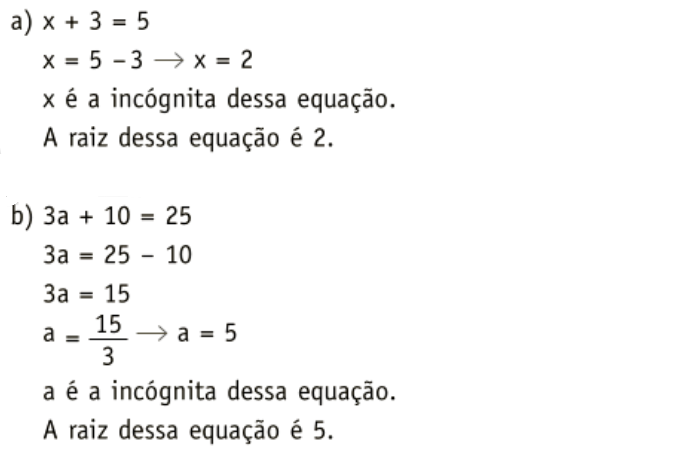
\includegraphics[scale=0.5]{def.png}

		\section*{Questões - Embasamento}
        
		\begin{enumerate}
			\item Determine a raiz das seguintes equações:
			\begin{enumerate}[label=(\alph*), itemsep=1em]
				\item $2x-4=8$
				\item $5a+5=20$
				\item $m+8=10$
				\item $10+8x=50$
				\item $x+8+3x=24$
				\item $y-12=8$
				\item $3k-2=25$
				\item $3x+8-x=10$
				\item $3a-12+a=12$
				\item $3w-14=6+w$ \\
			\end{enumerate}

			\item Determine o valor de x para que as expressões a seguir sejam verdadeiras:
			
			\begin{enumerate}[label=(\alph*), itemsep=1em]
				\item $x+3=5$
				\item $2x=8$
				\item $3x+1=10$
				\item $5-x=3$
				\item $3x+5=65$
				\item $4x+7=27$
				\item $5x+2=52$
				\item $2x-3=7$
				\item $7x-9=54$
				\item $8x-3=45$
			\end{enumerate}

			\item Resolva as seguintes equações:
			
			\begin{enumerate}[label=(\alph*), itemsep=1em]
				\item $2x+5=47-4x$
				\item $3(4-2x)=45-17x$
				\item $4y+18=72-2y$
				\item $30-4a=2(a-3)$
				\item $2(x+3)+4(x-2)=5(x-7)+2(x+3)$
				\item $\dfrac{3-x}{5}+1=\dfrac{x-4}{2}$
				\item $5+\left( x+\dfrac{x}{2} \right)=15$
				\item $12-x=\left( \dfrac{7}{5} \right) x$
				\item $x=4(5-x)$
				\item $x+2x+4x=70$
			\end{enumerate}

			\item Resolver as equações
			\begin{enumerate}[label=(\alph*), itemsep=1em]
				\item $4(3x-2)+5(7-2x)=15$
				\item $2(x+1)+3(x-2)=8x+7$
				\item $3a+2-4(a+3)=3(5-3a)$
				\item $4(1-m)=3-4(2-2m)$
				\item $2(1-4x)+3(2x-7)+4(x-5)=10$
				\item $(x+3)+(2x+6)+(3x+9)=36$
				\item $2(4-2x)+3(5-7x)=6(8-6x)$
				\item $(4m-3)+2(m+5)+3(m-7)=-70$
				\item $(z+5)3+(z+8)4=6z+13$
			\end{enumerate}

			\item Resolva as equações
			
			
			\begin{enumerate}[label=(\alph*), itemsep=1em]
				\item $\dfrac{x}{2}+\dfrac{1-x}{4}=\dfrac{x+1}{4}$
				\item $\dfrac{a}{3}+\dfrac{a}{6}=3$
				\item $\dfrac{x-2}{4}=x-8$
				\item $\dfrac{x-1}{2}=\dfrac{19-x}{4}$
				\item $\dfrac{x+1}{2}+\dfrac{x+1}{3}=20$
				\item $\dfrac{1}{2}+2x=x-\dfrac{1}{2}$
				\item $\dfrac{x-2}{319}=0$
				\item $\dfrac{415(x-3)}{777}=0$
				\item $\dfrac{x-1}{419^{2}+420^{2}}=0$
				\item $\dfrac{x-1}{2}+\dfrac{x-2}{3}+\dfrac{x-3}{4}=\dfrac{4}{3}$
			\end{enumerate}

			


		\end{enumerate}
	
\end{document}